\documentclass[border=4pt]{standalone}

\usepackage{tikz}

\definecolor{otblue}{HTML}{0072B2}
\definecolor{otorange}{HTML}{E69F00}
\definecolor{otteal}{HTML}{009E73}
\definecolor{otpurple}{HTML}{CC79A7}
\definecolor{otgray}{HTML}{5A5A5A}

\begin{document}
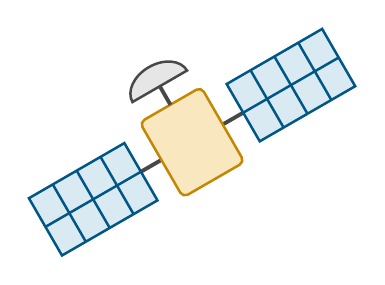
\begin{tikzpicture}[line width=0.9pt]
  \begin{scope}[rotate=30]
    \foreach \s in {-1,1}{
      \draw[otgray!80!black, line width=1.4pt] ({\s*0.45},0) -- ({\s*0.75},0);
      \filldraw[draw=otblue!75!black, fill=otblue!15] ({\s*0.75},-0.42) rectangle ({\s*2.15},0.42);
      \foreach \t in {1.1,1.45,1.8}{\draw[otblue!75!black] ({\s*\t},-0.42) -- ({\s*\t},0.42);}
      \draw[otblue!75!black] ({\s*0.75},0) -- ({\s*2.15},0);
    }
    \filldraw[draw=otorange!85!black, fill=otorange!25, rounded corners=2pt] (-0.45,-0.55) rectangle (0.45,0.55);
    \draw[otgray!80!black, line width=1.4pt] (0,0.55) -- (0,0.85);
    \filldraw[draw=otgray!80!black, fill=otgray!15] (-0.4,0.82) arc[start angle=180, end angle=360, x radius=0.4, y radius=-0.28] -- cycle;
  \end{scope}
\end{tikzpicture}
\end{document}
